%!TEX root = main.tex
\section{Introduction}% 
\par With the ever-increasing complexity and size of datasets, there is a growing demand for information visualization tools that help analysts make sense of large amounts of data. Visual data exploration is one of the most commonly used technique that powerfully couples human insights with statistical and data management solutions to help analysts rapidly generate hypothesis, discover interesting trends and patterns, and identify clusters and anomalies. In this paper, we present challenges in the various stages in the cycle of visual analysis, and discuss ongoing and future directions of research that addresses these issues.
% guides users through the acts of visual data exploration as shown in Figure~\ref{fig:cycle}, including searching for a precise visualizations, querying with a vague intent, and recommending visualizations that facilitates better data understanding and awareness. Our presentation of the spiral in Figure~\ref{fig:cycle} does not imply a monotonic sequences of actions, nor are the acts of visual data exploration mutually exclusive from one another, instead the diagram should read as a series of workflow that interleaves and forms an iterative cycle that reinforces one another. For example, as we will discuss in Section \ref{sec:hypothesis}, better data understanding can lead to better precise visual querying behaviors.
\begin{figure}[h!]
\label{fig:table}
\centering
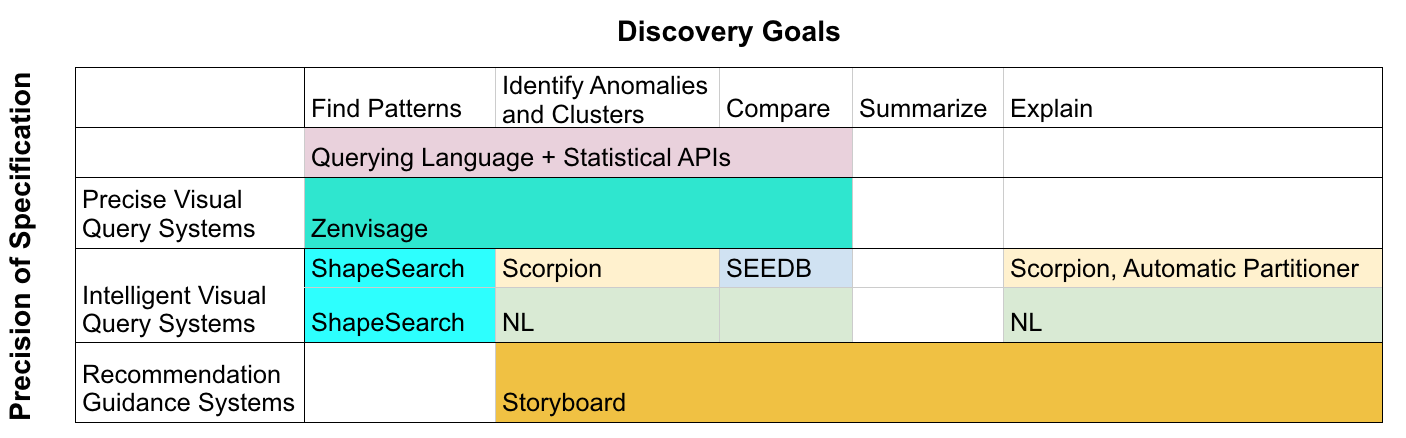
\includegraphics[width=0.7\linewidth]{figures/table.png}
\caption{Overview of the systems described in this paper. Columns are organized into discovery goals and rows are ordered by decreasing levels of query specificity and correspondingly increasing levels of autonomous assistance.}
\end{figure}
\par Our paper focuses on ongoing research in interactive systems that accelerates users towards common discovery goals in visual data exploration. On the horizontal axis of Figure \ref{fig:table}, we list five different common discovery goals in visual data exploration characterized by functionalities in existing systems and related works on visualization taxonomy\cite{Heer2012,Amar2005}. The table omits the description of low-level task (such as filtering, sorting), since these functionalities are seen as commonplace in popular data analytics tools such as Excel, Tableau. The vertical axis of the table characterizes the division of work between how much the user has to specify versus how much the system automatically infer and achieve the goals that they want to accomplish. At the topmost row, we find that while most discovery goals can be accomplished through exact and complete specification to query languages and programmatic APIs to statistical tools, these systems are often not easily accesible by non-experts.
% On the vertical axis, we describe systems with varying degree of query specificity. All discovery goals except for summarization and explaination could be performed through exact and complete specification to query languages and programmatic APIs to statistical tools. 
\par In Section \ref{sec:precise}, we discuss how precise visual query systems help accelerate the process of finding desired visualizations, which in turn facillitates other highlighted discovery goals. Precise visual query system addresses the common problem of having to manually examine large numbers of visualizations in search of a desired pattern, which can be error-prone and inefficient. We discuss our work on \zv which allows analysts to specify their desired visualization through front-end interactions and automatically returns a ranked list of visualizations that closely matches with the input query.
\par Examples from our \zv design study demonstrates that precise querying alone is insufficient for addressing all the visual querying demands required in real-world use cases. In addition, we find that users often do not have a good idea of what they want to query for without looking at example visualizations or summaries of the data. To bridge the gap between user's high-level intent and what the system operates as inputs, we advocate that future research needs to look beyond simple precise visual querying by : 1) making visual query system more expressive by supporting a wider class of vague queries (Section~\ref{sec:vague}) and 2) making it easier to know what to query by recommending visualizations that facilitate data awareness (Section~\ref{sec:understanding}).
\par Accordingly, the next row in the table highlights a growing class of \textit{intelligent visual querying system} (IVQS) that interprets the `vagueness' of queries and allow users to tweak or refine their queries through a feedback mechanism. \dor{I think we need to expand this definition depending on the new content that we will be adding, ShapeSearch, SeeDB, Scorpion?} 
\par To address the problem of guiding users to portions of the data that they might be interested in querying, Section~\ref{sec:understanding} introduces systems that help users become more aware of their dataset and visualize where they are in their analysis workflow. The challenge in building these systems involves understanding what types of visualizations should be recommended to facilitate data awareness. As an example, we describe our work on \sbd, a system that provides data summaries and guides users through informative subsets of data. Finally, we discuss related works on how visualizing provenance and situational information can guide users towards more informative analysis actions.
%The bottom-most row of the figure refers to recommendation systems that guide users towards better data understanding with minimial required inputs, as described in Section~\ref{sec:understanding}.
% \begin{figure}[h!]
% \label{fig:cycle}
% \centering
% 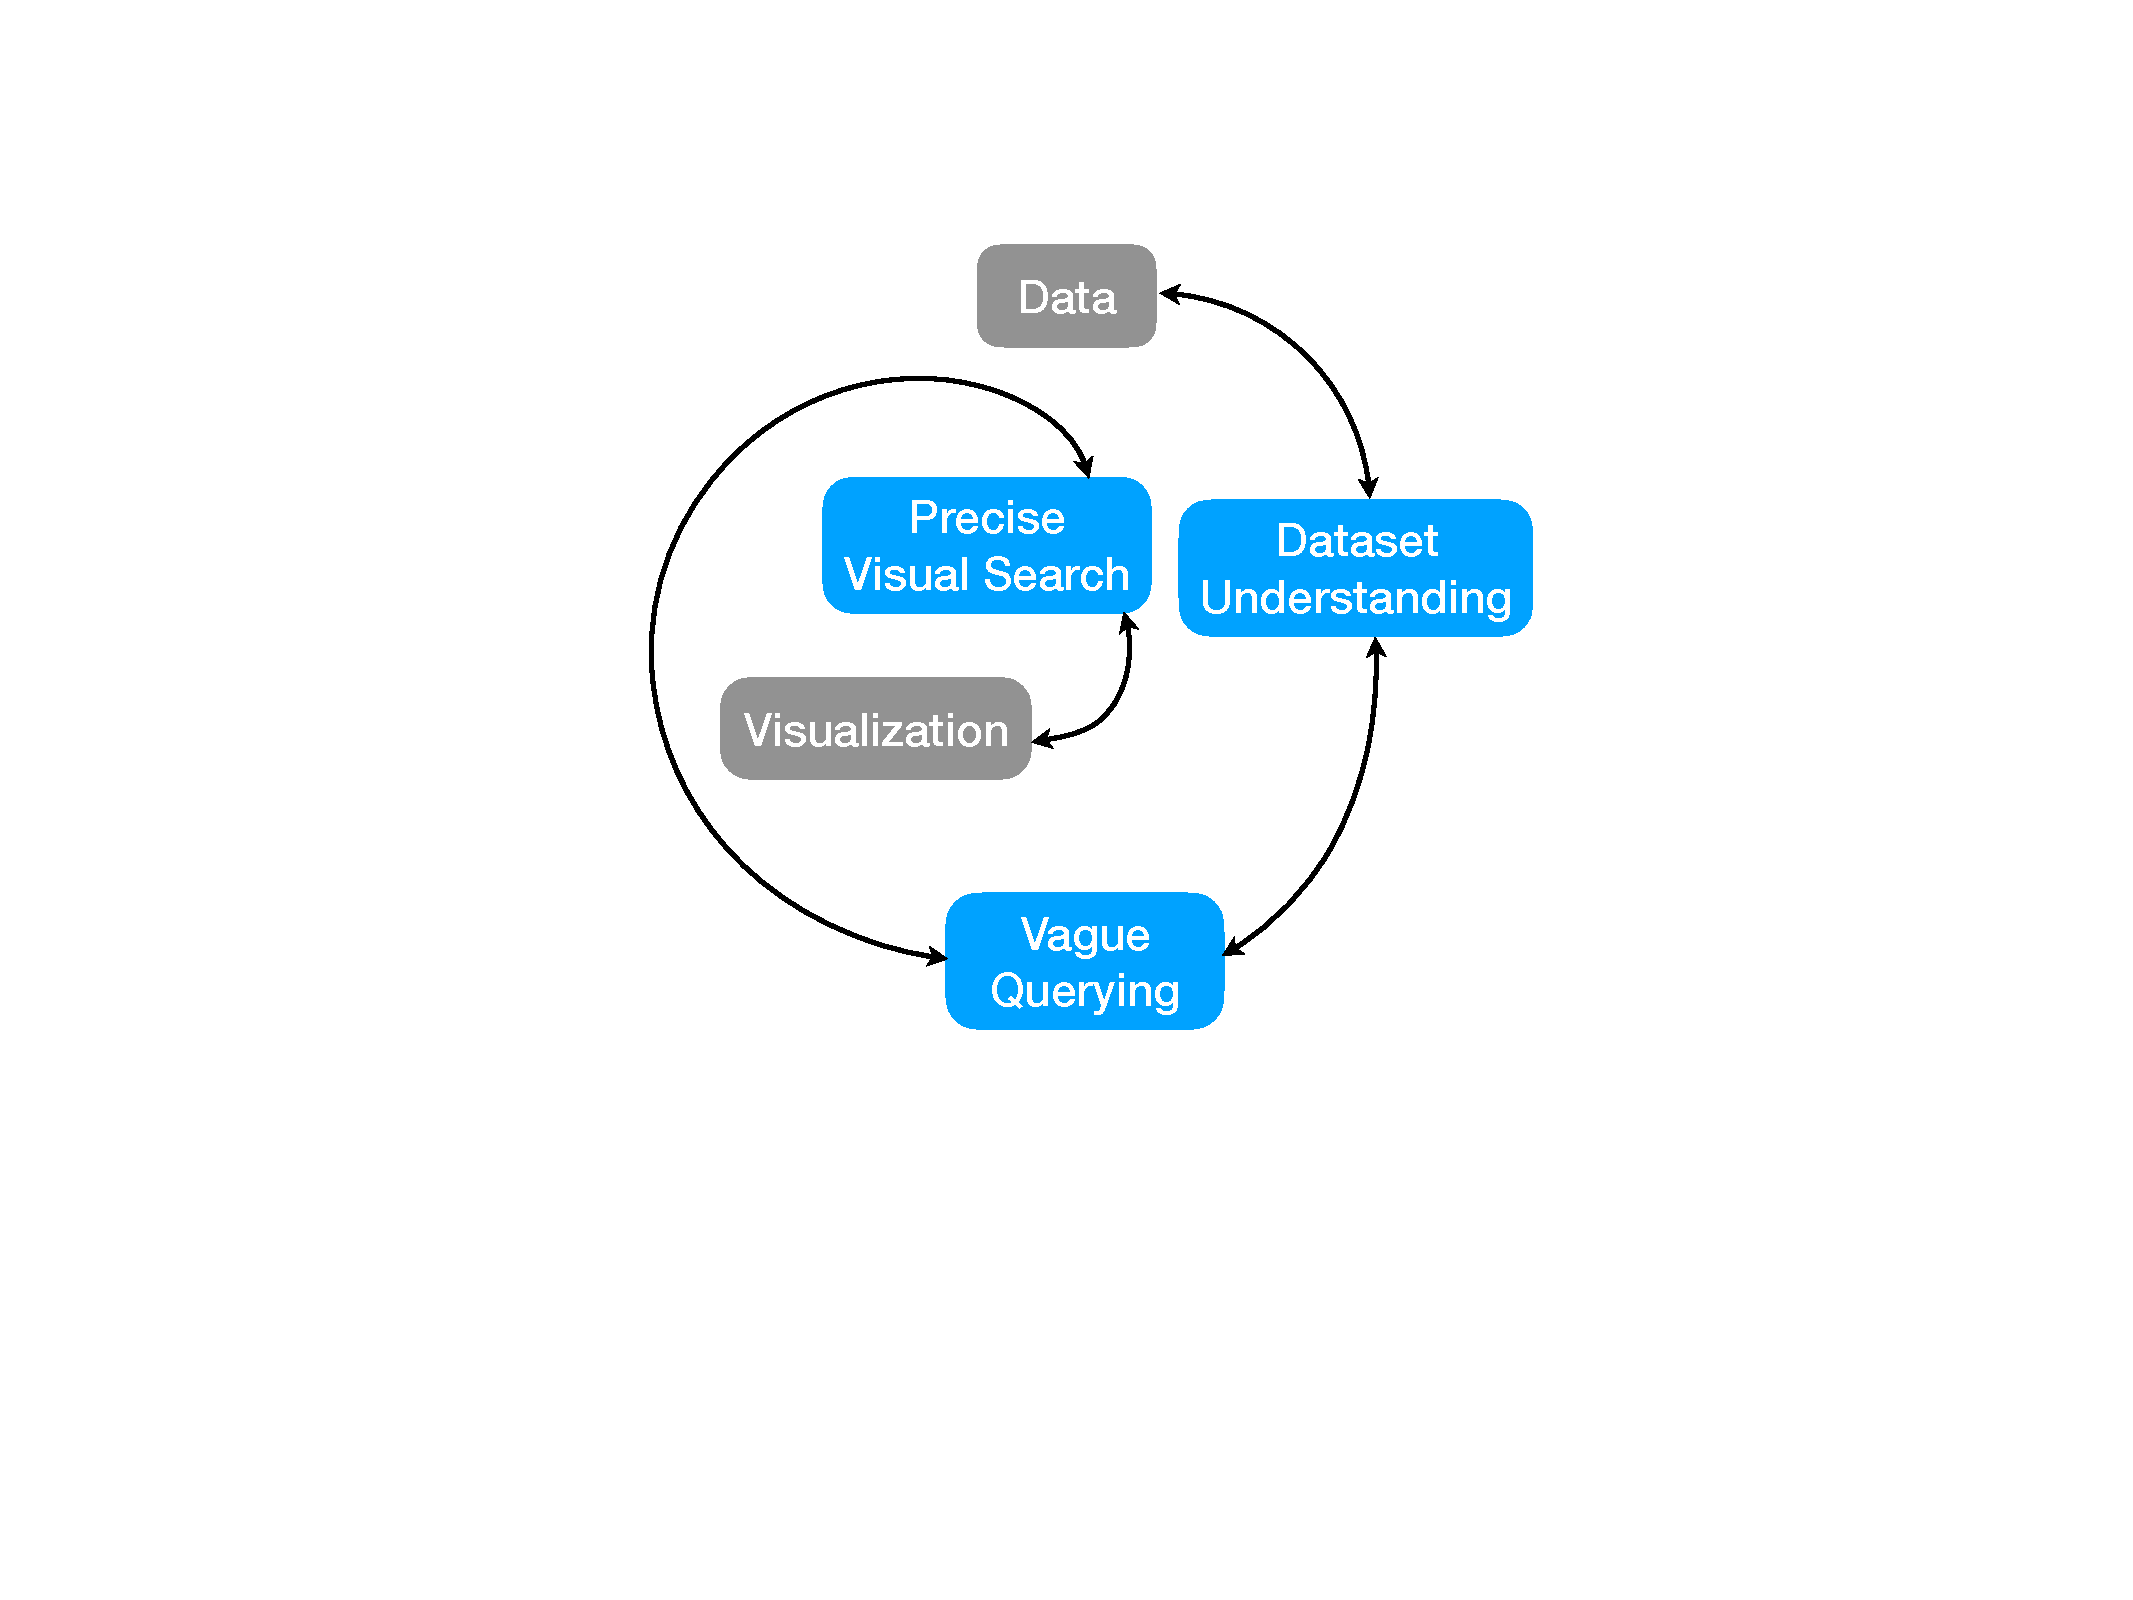
\includegraphics[width=0.4\linewidth]{figures/cycle.pdf}
% \caption{Cycle of visual data exploration.}
% \end{figure}
% “What is the problem”, “Why is this important”, “Why do previous approaches fail”, “Why is this hard”, “What is our approach” paragraphs into the intro
% \par Starting from the innermost spiral, 
% \par In Section~\ref{sec:precise}, we highlight examples from our \zv design study where precise querying alone is insufficient for addressing all the visual querying demands required in real-world use cases. In addition, we find that users often do not have a good idea of what they want to query for without looking at example visualizations or summaries of the data. To improve the flow of visual data exploration, we advocate to make visual query system more expressive by supporting a wider class of vague queries (Section~\ref{sec:vague}) and make it easier to know what to query by recommending visualizations that facilitate data awareness (Section~\ref{sec:understanding}).
% \par Section~\ref{sec:vague} explains why the trade-off between expressiveness and usability in most interactive analytics system is an inherent challenge in making visual query systems more expressive. We discuss a growing class of \textit{intelligent visual querying system} (IVQS) that tries to interpret the `vagueness' of queries and allow users to tweak or refine their queries through a feedback mechanism.
% \par To address the problem of guiding users to portions of the data that they might be interested in querying, Section~\ref{sec:understanding} introduces systems that help users become more aware of their dataset and visualize where they are in their analysis workflow. The challenge in building these systems involves understanding what types of visualizations should be recommended to facilitate data awareness. As an example, we describe our work on \sbd, a system that provides data summaries and guides users through informative subsets of data. Finally, we discuss related works on how visualizing provenance and situational information can guide users towards more informative analysis actions.
\par Our paper mainly focusses on the search and recommendation of visualization for data exploration, but also touches on related work in generic data querying. Related works on recommendation and automatic selection of the visualization design and encoding~\cite{Wongsuphasawat2017,Mackinlay2007} as well as frameworks and grammar for interactive visualization (Vega, D3) is out of the scope of this paper.

% graphical presentation (ShowMe, Voyager, etc) as well as declarative specification of interactive visualization (Vega-lite, D3 papers, cite Heer and Shneiderman) is out of scope of this ---.  
% For a more detailed survey --- , see ----\cite{Heer2012,}. 
%, so that analysts can make more informed analysis decisions subsequently
% Visualization ---> insights. 
% \begin{enumerate}
% 	\item Visual analysis help discover insights, etc.
% 	\item supporting cycle of visual data exploration. 
% 	\item In this paper, we introduce various challenges in the ---- visual analysis, and discuss ---- solutions ---.
% 	\item Challenge \#1: Precise search
% 		\item finding the right vis and relevant data is hard, 
% 		\item  we discuss \zv as one use case and solution in this space (Section \ref{sec:precise})
% 	\item Challenge \#2: Need for in-the-loop support. how do people query visually? 
% 		\item During our PD + others, hypothesis + in the loop considerations is important. We discuss relevant work and our findings in Section \ref{sec:hypothesis}.
% 		\item Need to formulate complex expressive queries, language is good, but need interface (e..g visual primitives) to support this. (Section \ref{sec:vague})
% 		\item top-down, bottom-up --> point to need for bottom-up recommendations (Section \ref{sec:understanding})
% 	\item Challenge \#3: Vague and intelligent search 
% 		\item Users might not always have something they want to start with, supporting vague querying (Section~\ref{sec:vague})
% 	\item Challenge \#4: Cold-start recommendation for data understanding. One aspect of this is to gain understanding of dataset, (e.g. representative and outliers in \zv, bottom up exploration)we discuss \sbd as one example solution addressing this problem (Section \ref{sec:understanding}).
% \end{enumerate}{}
%, including searching for patterns, identifying clusters and anomalies, compare, summarize, and explain, ince we wanted to --- high-level goals ---discovery, 
